\section{Model}
\label{sec:model}

In this paper, we propose a neural and probabilistic framework to generate
descriptions from images. Recent advances in statistical machine
translation have shown that, given a powerful sequence model, it is
possible to achieve state-of-the-art results by directly maximizing
the probability of the correct translation given an input sentence in
an ``end-to-end'' fashion -- both for training and inference. These
models make use of a recurrent neural network
which encodes the variable length input into a fixed dimensional
vector, and uses this representation to ``decode'' it to the desired
output sentence. Thus, it is natural to use the same approach where,
given an image (instead of an input sentence in the source language),
one applies the same principle of ``translating'' it into its
description.

Thus, we propose to directly maximize the probability of the correct
description given the image by using the following formulation:

\begin{equation}
\theta^\star = \arg\max_\theta \sum_{(I,S)} \log p(S | I ; \theta)
\label{eqn:obj}
\end{equation}
where $\theta$ are the parameters of our model, $I$ is an image, and
$S$ its correct transcription. Since $S$ represents any sentence, its
length is unbounded. Thus, it is common to apply the chain rule to
model the joint probability over $S_0,\ldots,S_N$, where $N$ is the
length of this particular example as

\begin{equation}
\log p(S | I) = \sum_{t=0}^N \log p(S_t | I, S_0, \ldots, S_{t-1})
\label{eqn:chain}
\end{equation}
where we dropped the dependency on $\theta$ for convenience.
At training
time, $(S,I)$ is a training example pair, and we optimize the sum of
the log probabilities as described in~(\ref{eqn:chain}) over the
whole training set using stochastic gradient descent (further training
details are given in Section \ref{sec:exps}).

It is natural to model $p(S_t | I, S_0, \ldots, S_{t-1})$ with a
Recurrent Neural Network (RNN), where the variable number of 
words we condition upon up to $t-1$ is expressed by a fixed length 
hidden state or memory $h_t$. This memory is updated after seeing a
new input $x_t$  by using a non-linear function $f$:
\begin{equation}\label{eq:rnn}
h_{t+1} = f(h_{t}, x_t)\;.
\end{equation}
To make the above RNN more concrete two crucial design choices are to be made: what is
the exact form of $f$ and how are the images and words fed as inputs $x_t$. For 
$f$ we use a Long-Short Term Memory (LSTM) net, which has shown state-of-the art
performance on sequence tasks such as translation. This model is outlined in the
next section. 

For the representation of images, we use a Convolutional Neural Network
(CNN). They have been widely used and studied for image tasks, and are
currently state-of-the art for object recognition and detection. Our particular
choice of CNN uses a novel approach to batch normalization and yields the
current best performance on the ILSVRC 2014 classification
competition~\cite{batchnorm}. Furthermore, they have been shown to
generalize to other tasks such as scene classification by means of
transfer learning~\cite{decaf2014}. The words are represented with an embedding
model.

\subsection{LSTM-based Sentence Generator}
\label{sec:lstm}

The choice of $f$ in (\ref{eq:rnn}) is governed by its 
ability to deal with vanishing and exploding gradients~\cite{hochreiter1997long},
the most common
challenge in designing and training RNNs. To address this challenge, a  particular form 
of recurrent nets, called LSTM, was introduced \cite{hochreiter1997long}
and applied with great success to translation \cite{cho2014learning,sutskever2014sequence} and sequence generation \cite{graves2013generating}.

\begin{figure}
\begin{center}
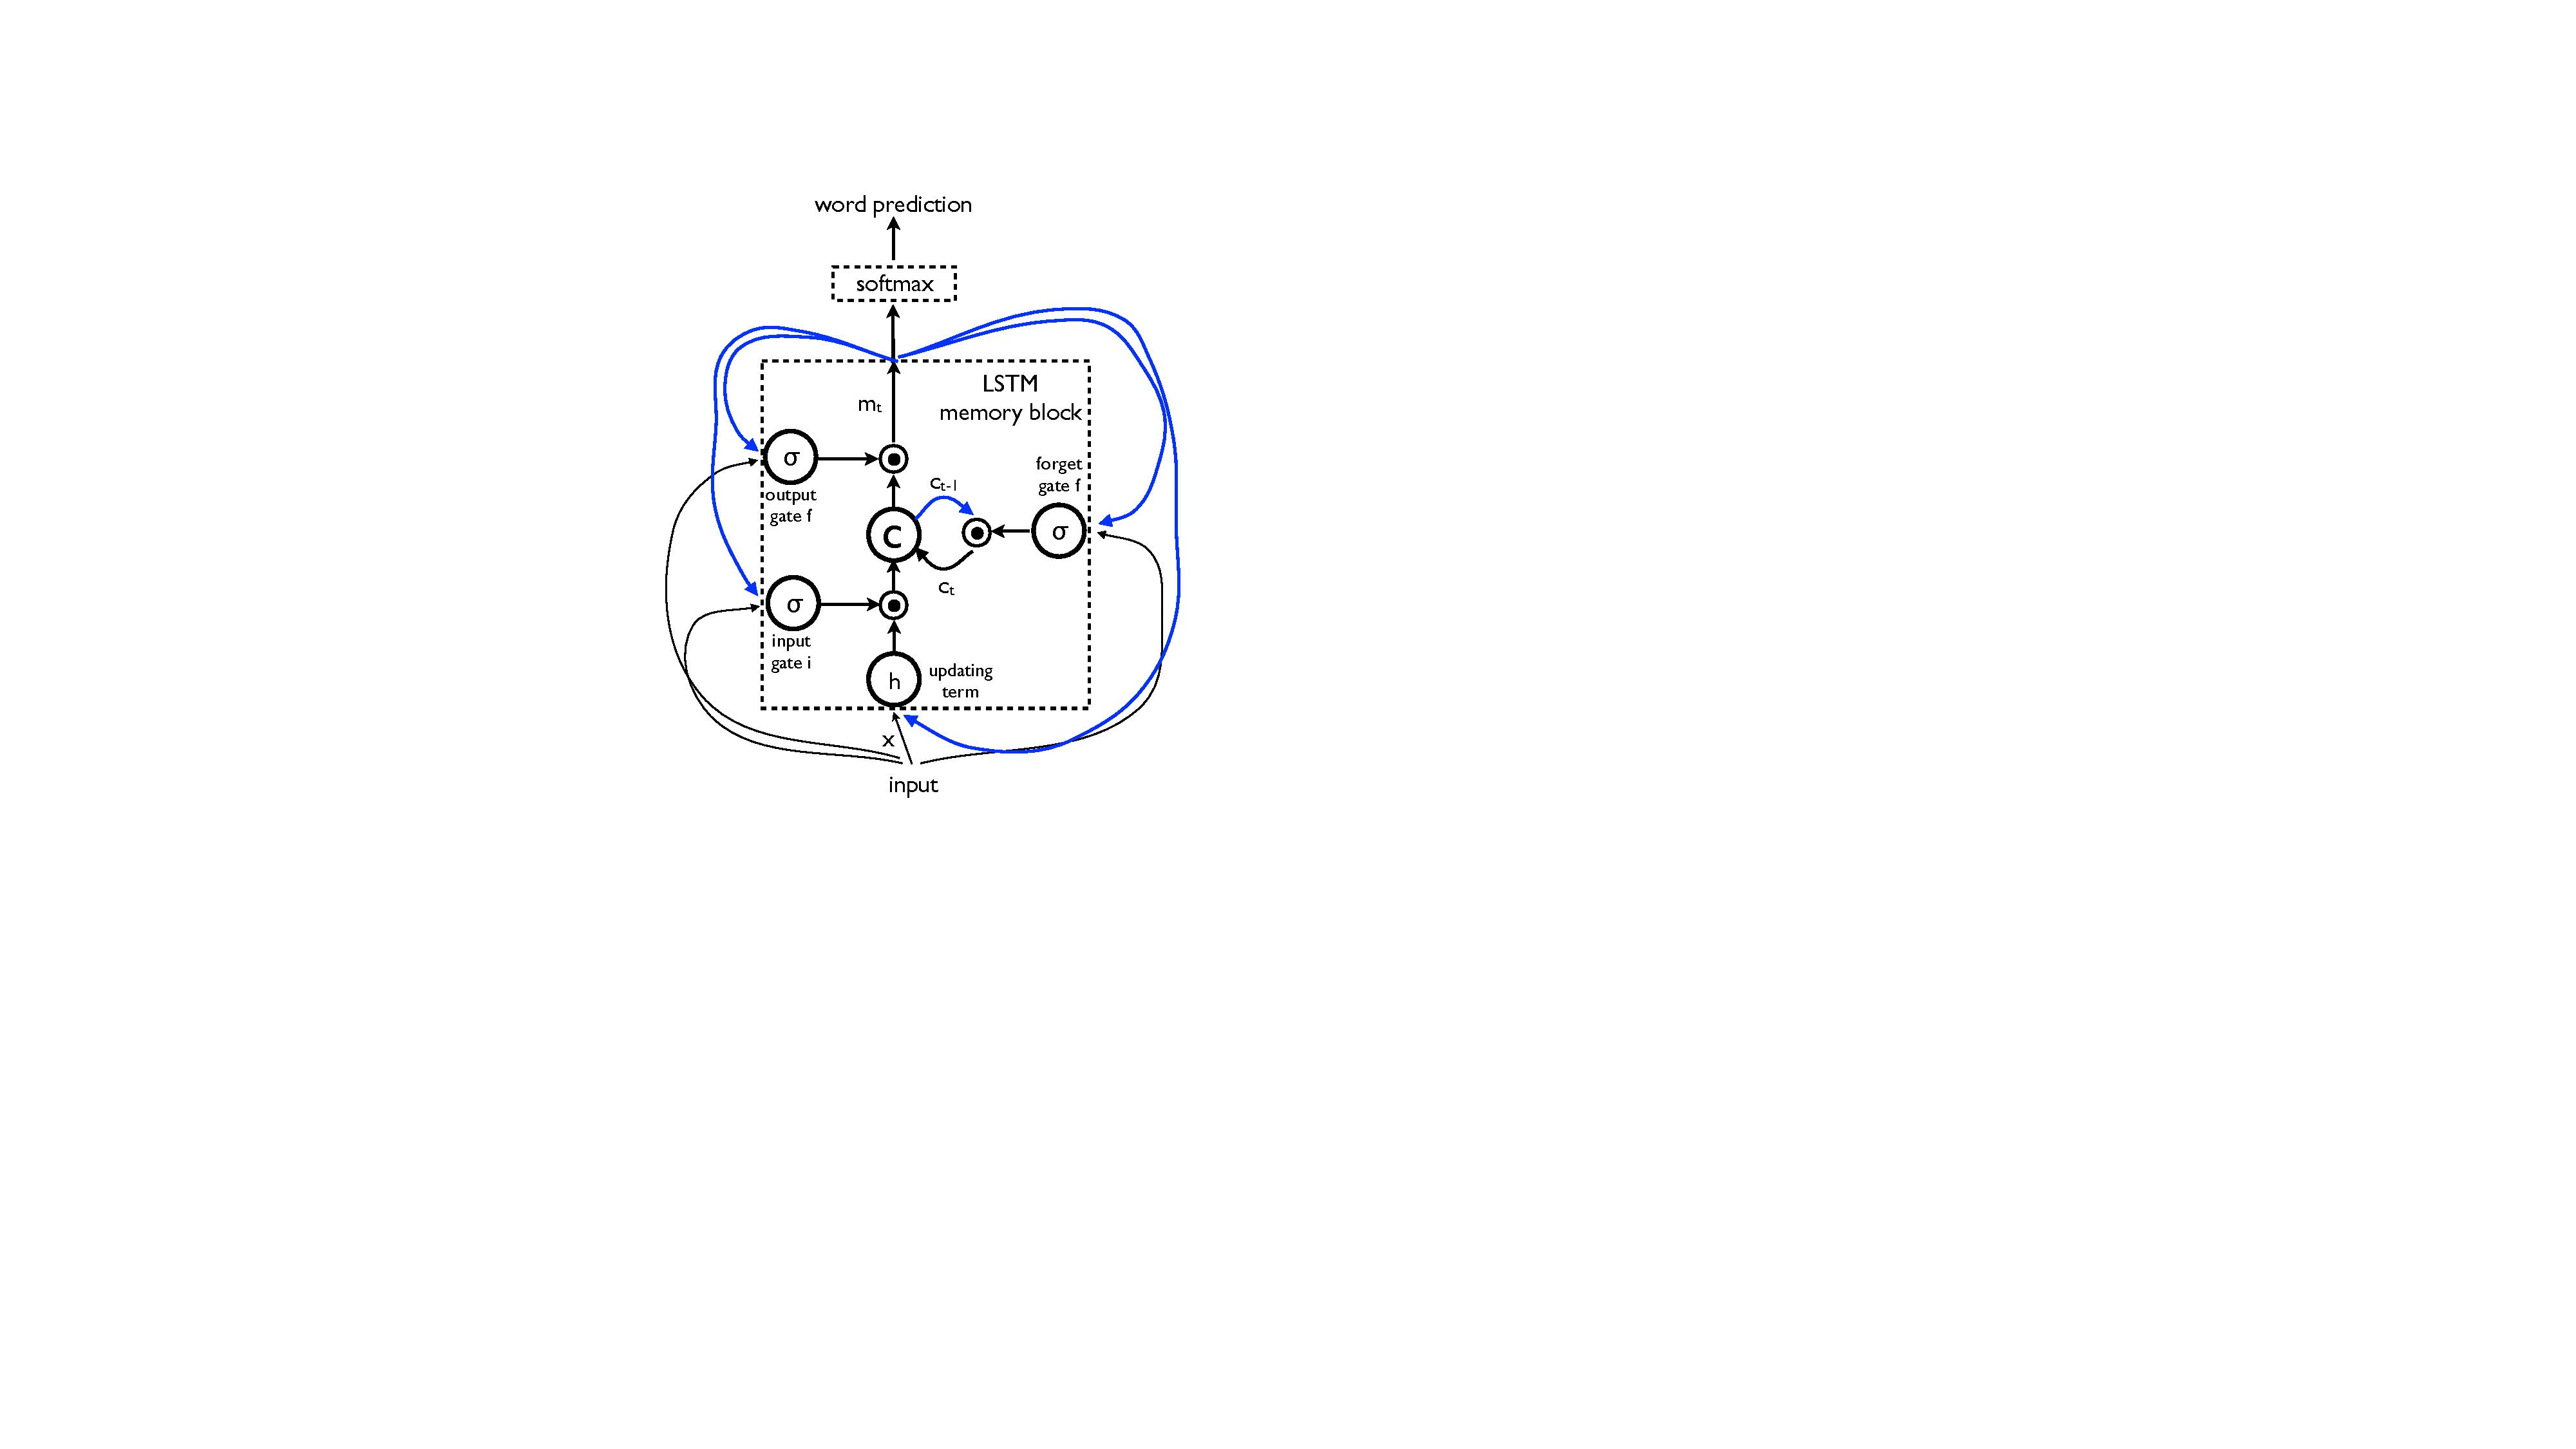
\includegraphics[width=0.85\columnwidth]{detailed_lstm_figure.pdf}
\end{center}
\caption{\label{fig:lstm} LSTM: the memory block contains a cell $c$ which is controlled by three gates. In blue we show the recurrent connections -- the output $m$ at time $t-1$ is fed back to the memory at time $t$ via the three gates; the cell value is fed back via the forget gate; the predicted word at time $t-1$ is fed back in addition to the memory output $m$ at time $t$ into the Softmax for word prediction.}
\end{figure}

The core of the LSTM model is a memory cell $c$ encoding
knowledge at every time step of what inputs have been observed up to this step (see Figure~\ref{fig:lstm}) . The behavior of the cell
is controlled by ``gates" -- layers which are applied multiplicatively and thus can
either keep a value from the gated layer if the gate is $1$ or zero this value if the gate is $0$.
In particular, three gates are being used which control whether to forget the current cell value (forget gate $f$),
if it should read its input (input gate $i$) and whether to output the new cell value (output gate $o$).
The definition of the gates and cell update and output are as follows:
\begin{eqnarray}
i_t &= &\sigma(W_{ix} x_t+ W_{im} m_{t-1}) \\
f_t  &= & \sigma(W_{fx} x_t+ W_{fm} m_{t-1}) \\
o_t  &= & \sigma(W_{ox} x_t + W_{om} m_{t-1})  \\
c_t  &= & f_t \odot c_{t-1} + i_t \odot h(W_{cx} x_t + W_{cm} m_{t-1}) \\
m_t  &= & o_t \odot c_t \\
p_{t+1} &=& \textrm{Softmax}(m_t) 
\end{eqnarray}
where $\odot$ represents the product with a gate value, and the various $W$
matrices are trained parameters. Such multiplicative gates make it
possible to train the LSTM robustly as these gates deal well with exploding and vanishing gradients \cite{hochreiter1997long}.
The nonlinearities are sigmoid $\sigma(\cdot)$ and hyperbolic tangent $h(\cdot)$.
The last equation $m_t$ is what is used
to feed to a Softmax, which will produce a probability distribution $p_t$ over all words.

\begin{figure}
\begin{center}
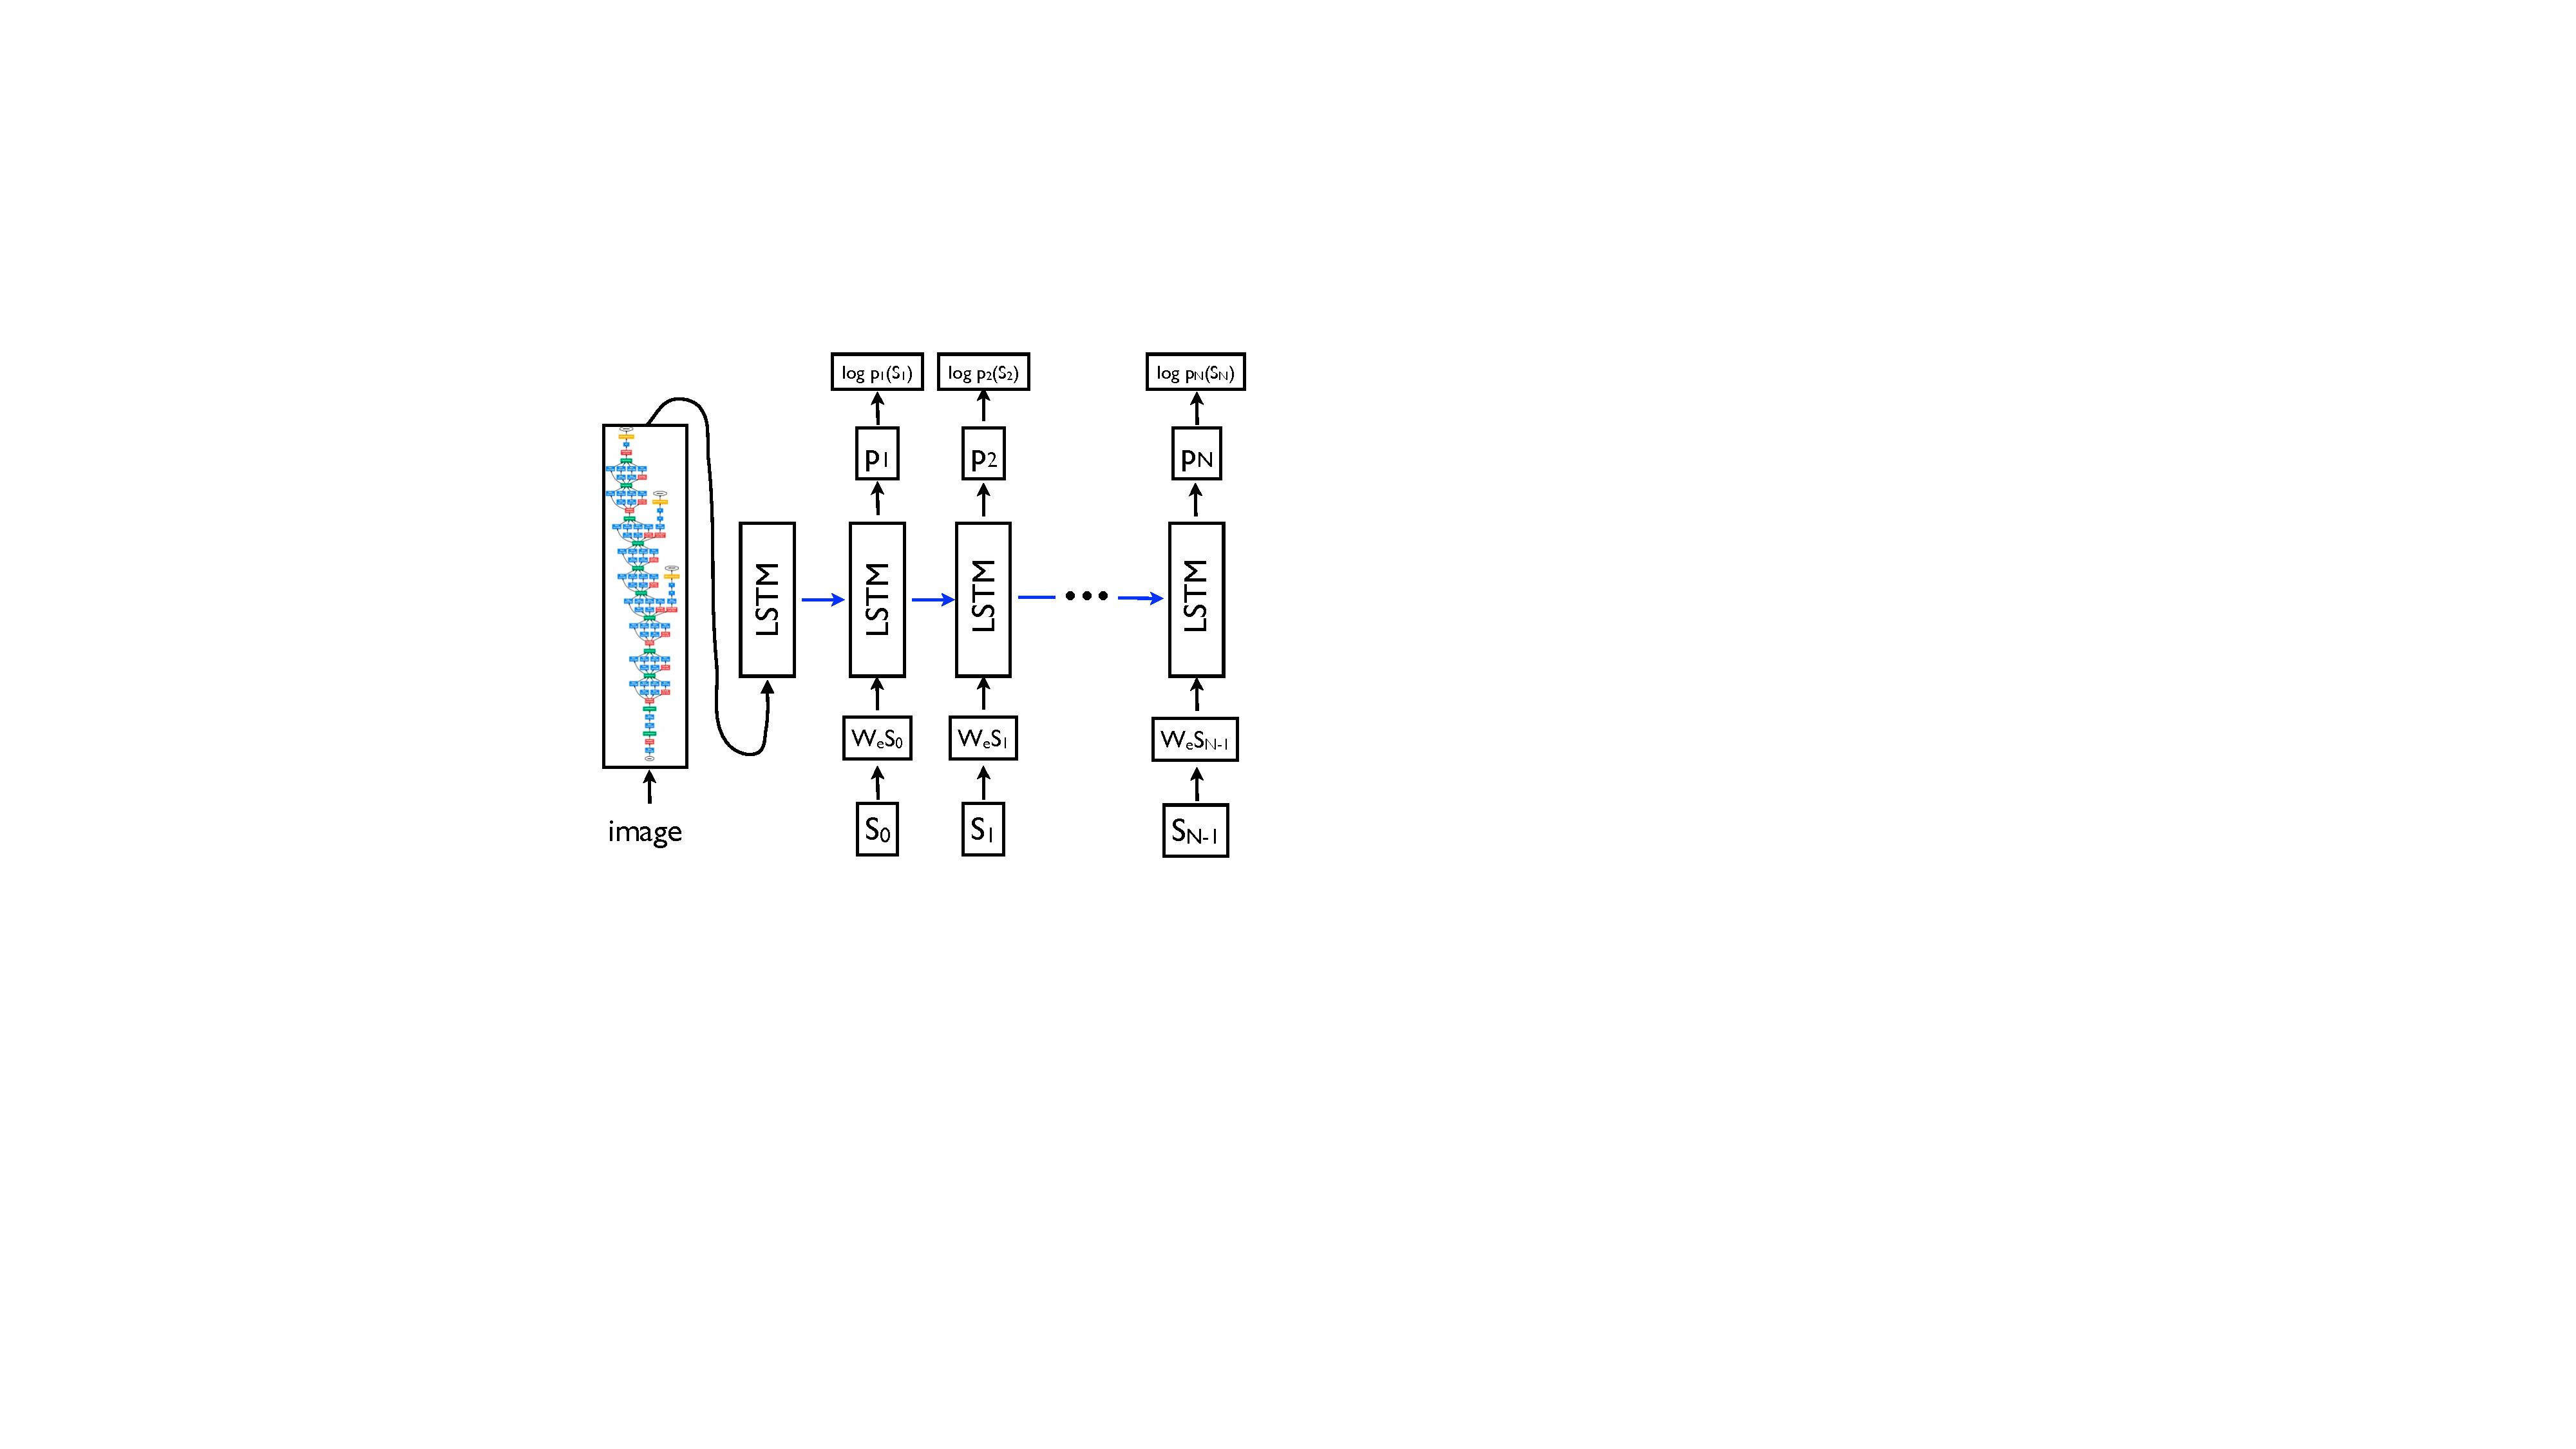
\includegraphics[width=0.75\columnwidth]{unrolled_lstm.pdf}
\end{center}
\caption{\label{fig:unrolled_lstm} LSTM model combined with a CNN image embedder (as defined in \cite{batchnorm}) and word embeddings. The unrolled connections between the LSTM memories are in blue and they correspond to the recurrent connections in Figure~\ref{fig:lstm}. All LSTMs share the same parameters. }
\end{figure}
\paragraph{Training} The LSTM model is trained to predict each word of the
sentence after it has seen the image as well as all preceding words as defined by
$p(S_t | I, S_0, \ldots, S_{t-1})$. For this purpose, it is instructive to think
of the LSTM in unrolled form -- a copy of the LSTM memory is created for the
image and each sentence word such that all LSTMs share the same parameters and the
output $m_{t-1}$ of the LSTM at time $t-1$ is fed to the LSTM at time $t$ (see
Figure~\ref{fig:unrolled_lstm}). All recurrent connections are transformed to feed-forward connections in the 
unrolled version. In more detail, if we denote by $I$ the input
image and by $S=(S_0,\ldots, S_N)$ a true sentence describing this image, the
unrolling procedure reads:
\begin{eqnarray}
x_{-1} &=& \textrm{CNN}(I)\\
x_t &=& W_e S_t, \quad t\in\{0\ldots N-1\}\quad \label{eqn:sparse}\\
p_{t+1} &=& \textrm{LSTM}(x_t), \quad t\in\{0\ldots N-1\}\quad
\end{eqnarray}
where we represent each word as a one-hot vector $S_t$ of dimension equal to the
size of the dictionary. Note that we denote by $S_0$ a special start word and by
$S_{N}$ a special stop word which designates the start and end of the sentence.
In particular by emitting the stop word the LSTM signals that a complete sentence
has been generated. Both the image and the words are mapped to the same space,
the image by using a vision CNN, the words by using word embedding $W_e$. The image
$I$ is only input once, at $t=-1$, to inform the LSTM about the image contents. We
empirically verified that feeding the image at each time step as an extra input yields
inferior results, as the network can explicitly exploit noise in the image and
overfits more easily.

Our loss is the sum of the negative log likelihood of the correct word at each step as follows:
\begin{equation}
L(I, S) = - \sum_{t=1}^N \log p_t(S_t) \; .
\end{equation}
The above loss is minimized w.r.t. all the parameters of the LSTM, the top layer of the
image embedder CNN and word embeddings $W_e$.

\paragraph{Inference}

There are multiple approaches that can be used to generate a sentence given
an image, with NIC. The first one is {\bf Sampling} where we just
sample the first word according to $p_1$, then provide the corresponding
embedding as input and sample $p_2$, continuing like this until we sample the
special end-of-sentence token or some maximum length.
The second  one is {\bf BeamSearch}: iteratively
consider the set of the $k$ best sentences up to time
$t$ as candidates to generate sentences of size $t+1$, and keep only the
resulting best $k$ of them. This better approximates
$S = \arg\max_{S'} p(S'|I)$.
We used the BeamSearch approach in the following experiments, with a
beam of size 20. Using a beam size of 1 (i.e., greedy search) did degrade our
results by 2 BLEU points on average.

